\section{Case Study: CDS-ASR}

CDS-ASR is used here only as a case study for aggregate-only reproducibility. The companion Paper 4-a carries the speech-evaluation method and CEIS technical claims.

The case has four evidence layers: a 258-row ASR split, selected-300 enriched high-stakes provenance outputs, a completed 300-row dual-reviewer human audit, and 900 model-row assessments per reviewer. Figure~\ref{fig:case_ladder} shows the case-study evidence ladder.

\begin{figure}[htbp]
\centering
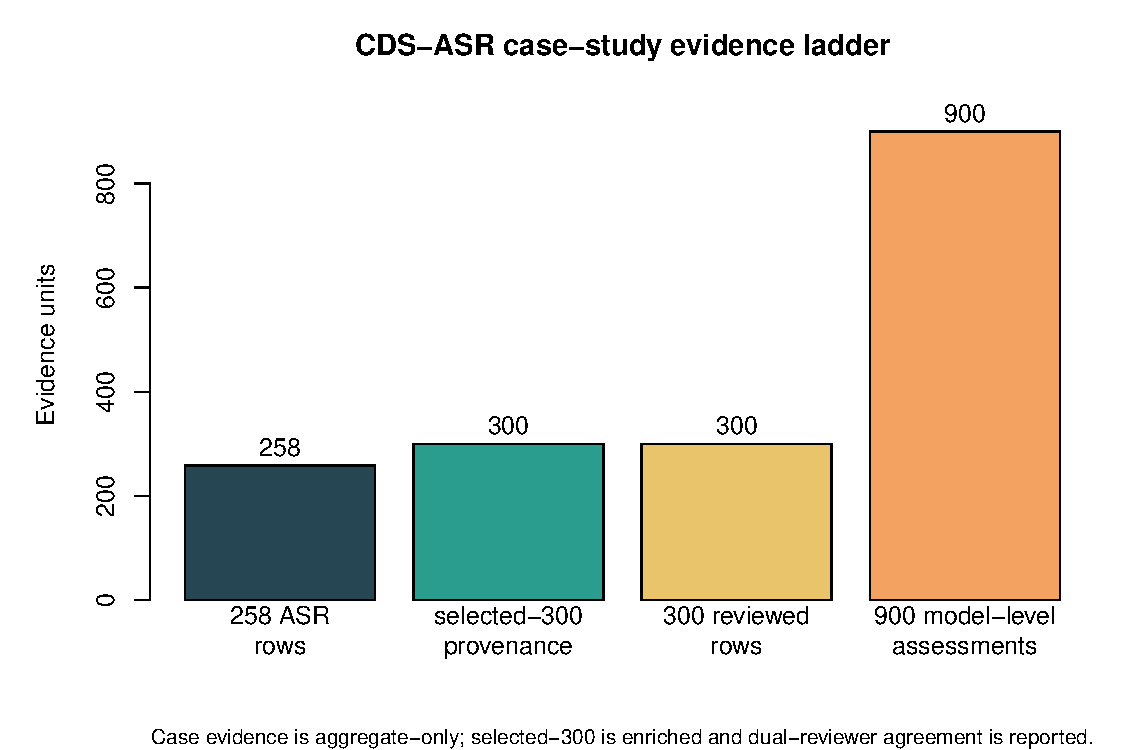
\includegraphics[width=.9\linewidth]{figures/fig5_case_study_evidence_ladder.pdf}
\caption{CDS-ASR case-study evidence ladder. Generated by \artifact{paper_4b_aggregate_reproducibility/r/build_fig5_case_study_evidence_ladder.R}.}
\label{fig:case_ladder}
\end{figure}

Predictor comparison, reviewer agreement, and policy replay appear as aggregate outputs. Raw audio, raw transcripts, row identifiers, reviewer notes, response sheets, model hypotheses, and transcript-bearing logs remain local-only. This makes the case appropriate for demonstrating reviewer-auditable aggregate evidence while preserving sensitive material.
